% ---------------------------------------------------------------------------
%  Appendices, in the order prescribed by the departmental template:
%    A  Plagiarism report front page
%    B  Paper publication details
%    C  Paper copy
%    D  Code snippets of major modules
%  Appendix headings are centred, "APPENDIX - X" over the title, as in the
%  template; the TOC entries are formatted by \appendixtocformat in report.tex.
% ---------------------------------------------------------------------------
\makeatletter
\renewcommand{\@makechapterhead}[1]{%
  \vspace*{10\p@}%
  {\centering\normalfont
    \ifnum\c@secnumdepth>\m@ne
      {\Large\bfseries APPENDIX - \thechapter\par}\nobreak
      \vskip 10\p@
    \fi
    \interlinepenalty\@M
    {\Large\bfseries\MakeUppercase{#1}\par}\nobreak
    \vskip 24\p@
  \par}}
\makeatother

% Plain code style for snippets: no frame, no numbers, no colour, as in the template.
\lstdefinestyle{snippet}{
  language=Python,
  basicstyle=\ttfamily\footnotesize,
  keywordstyle=\ttfamily,
  commentstyle=\ttfamily,
  stringstyle=\ttfamily,
  identifierstyle=\ttfamily,
  backgroundcolor=\color{white},
  frame=none,
  numbers=none,
  xleftmargin=0pt,
  aboveskip=6pt,
  belowskip=12pt,
  columns=fullflexible,
  keepspaces=true,
  breaklines=true,
  showstringspaces=false,
}
% \snippet{title}{file path}{location inside the file}
\newcommand{\snippet}[3]{%
  \par\vspace{0.6em}\noindent\textbf{#1}\par
  {\sloppy\noindent\itshape Source: \code{#2}, #3.\par}}

% ===========================================================================
\chapter[Plagiarism Report Front Page]{Plagiarism Report Front Page}
\thispagestyle{plain}

\begin{center}
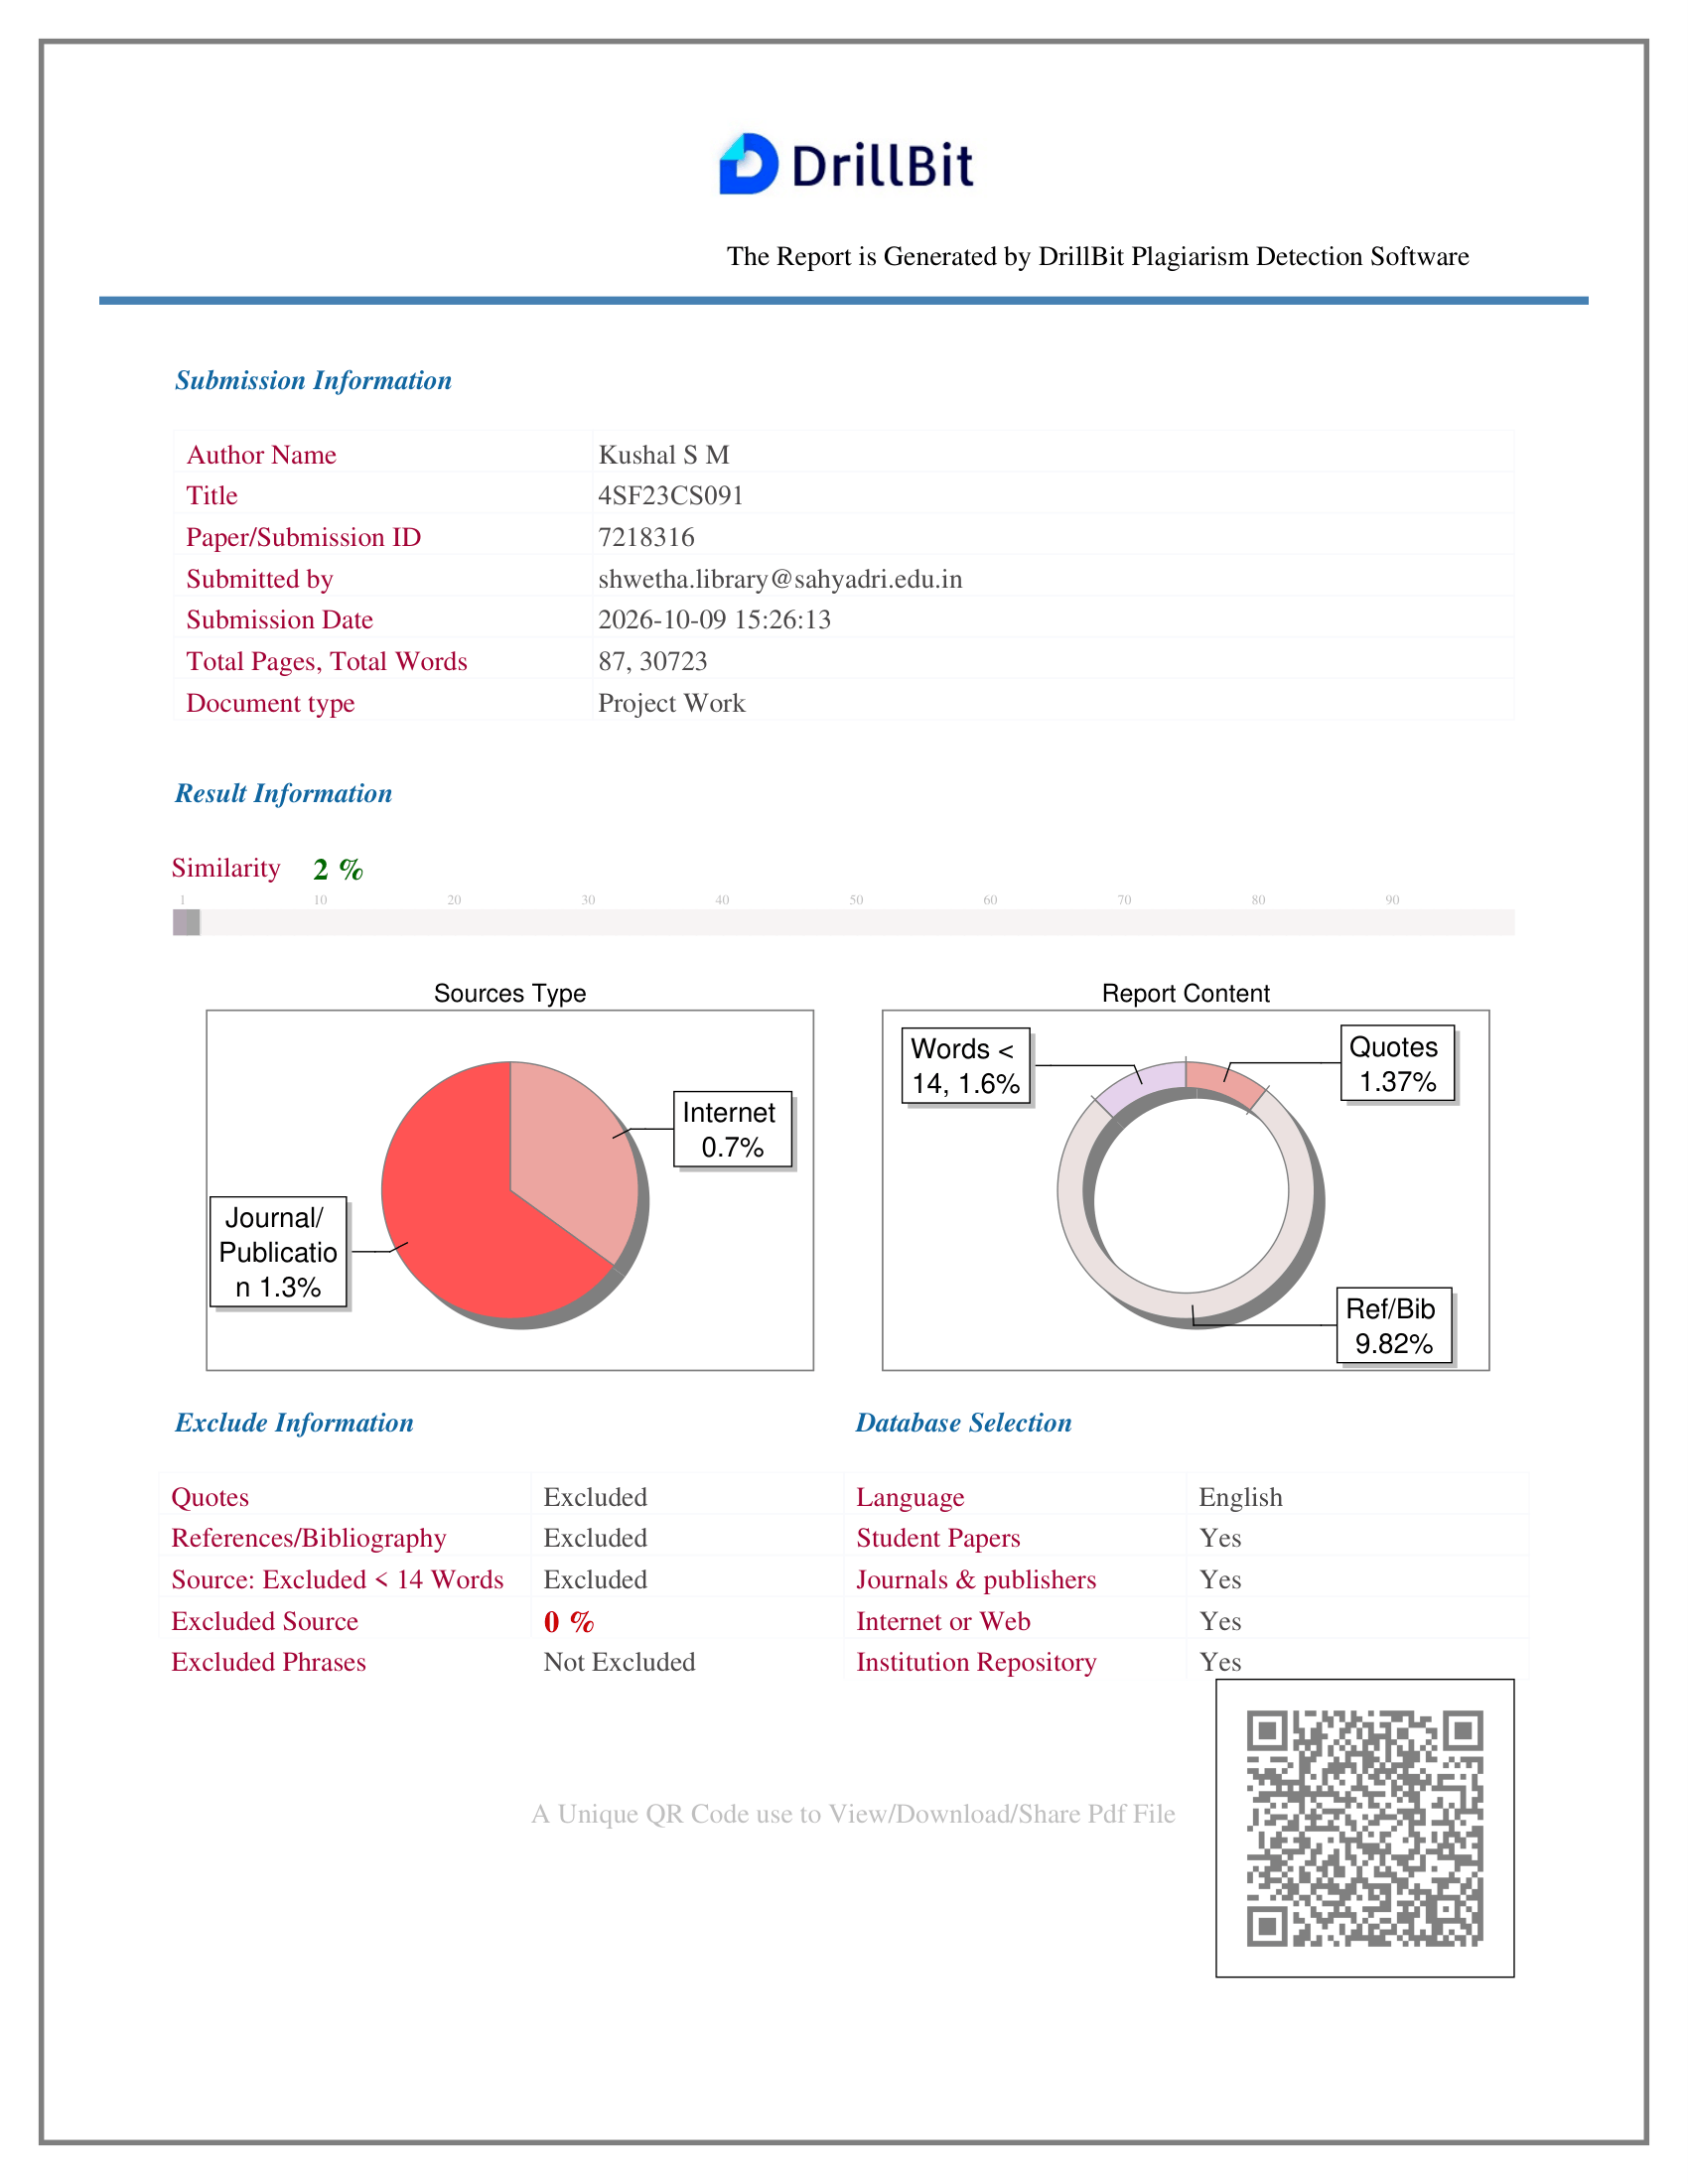
\includegraphics[width=\textwidth,height=0.72\textheight,keepaspectratio]{similarity}
\end{center}

\clearpage
\thispagestyle{plain}
\begin{center}
\fbox{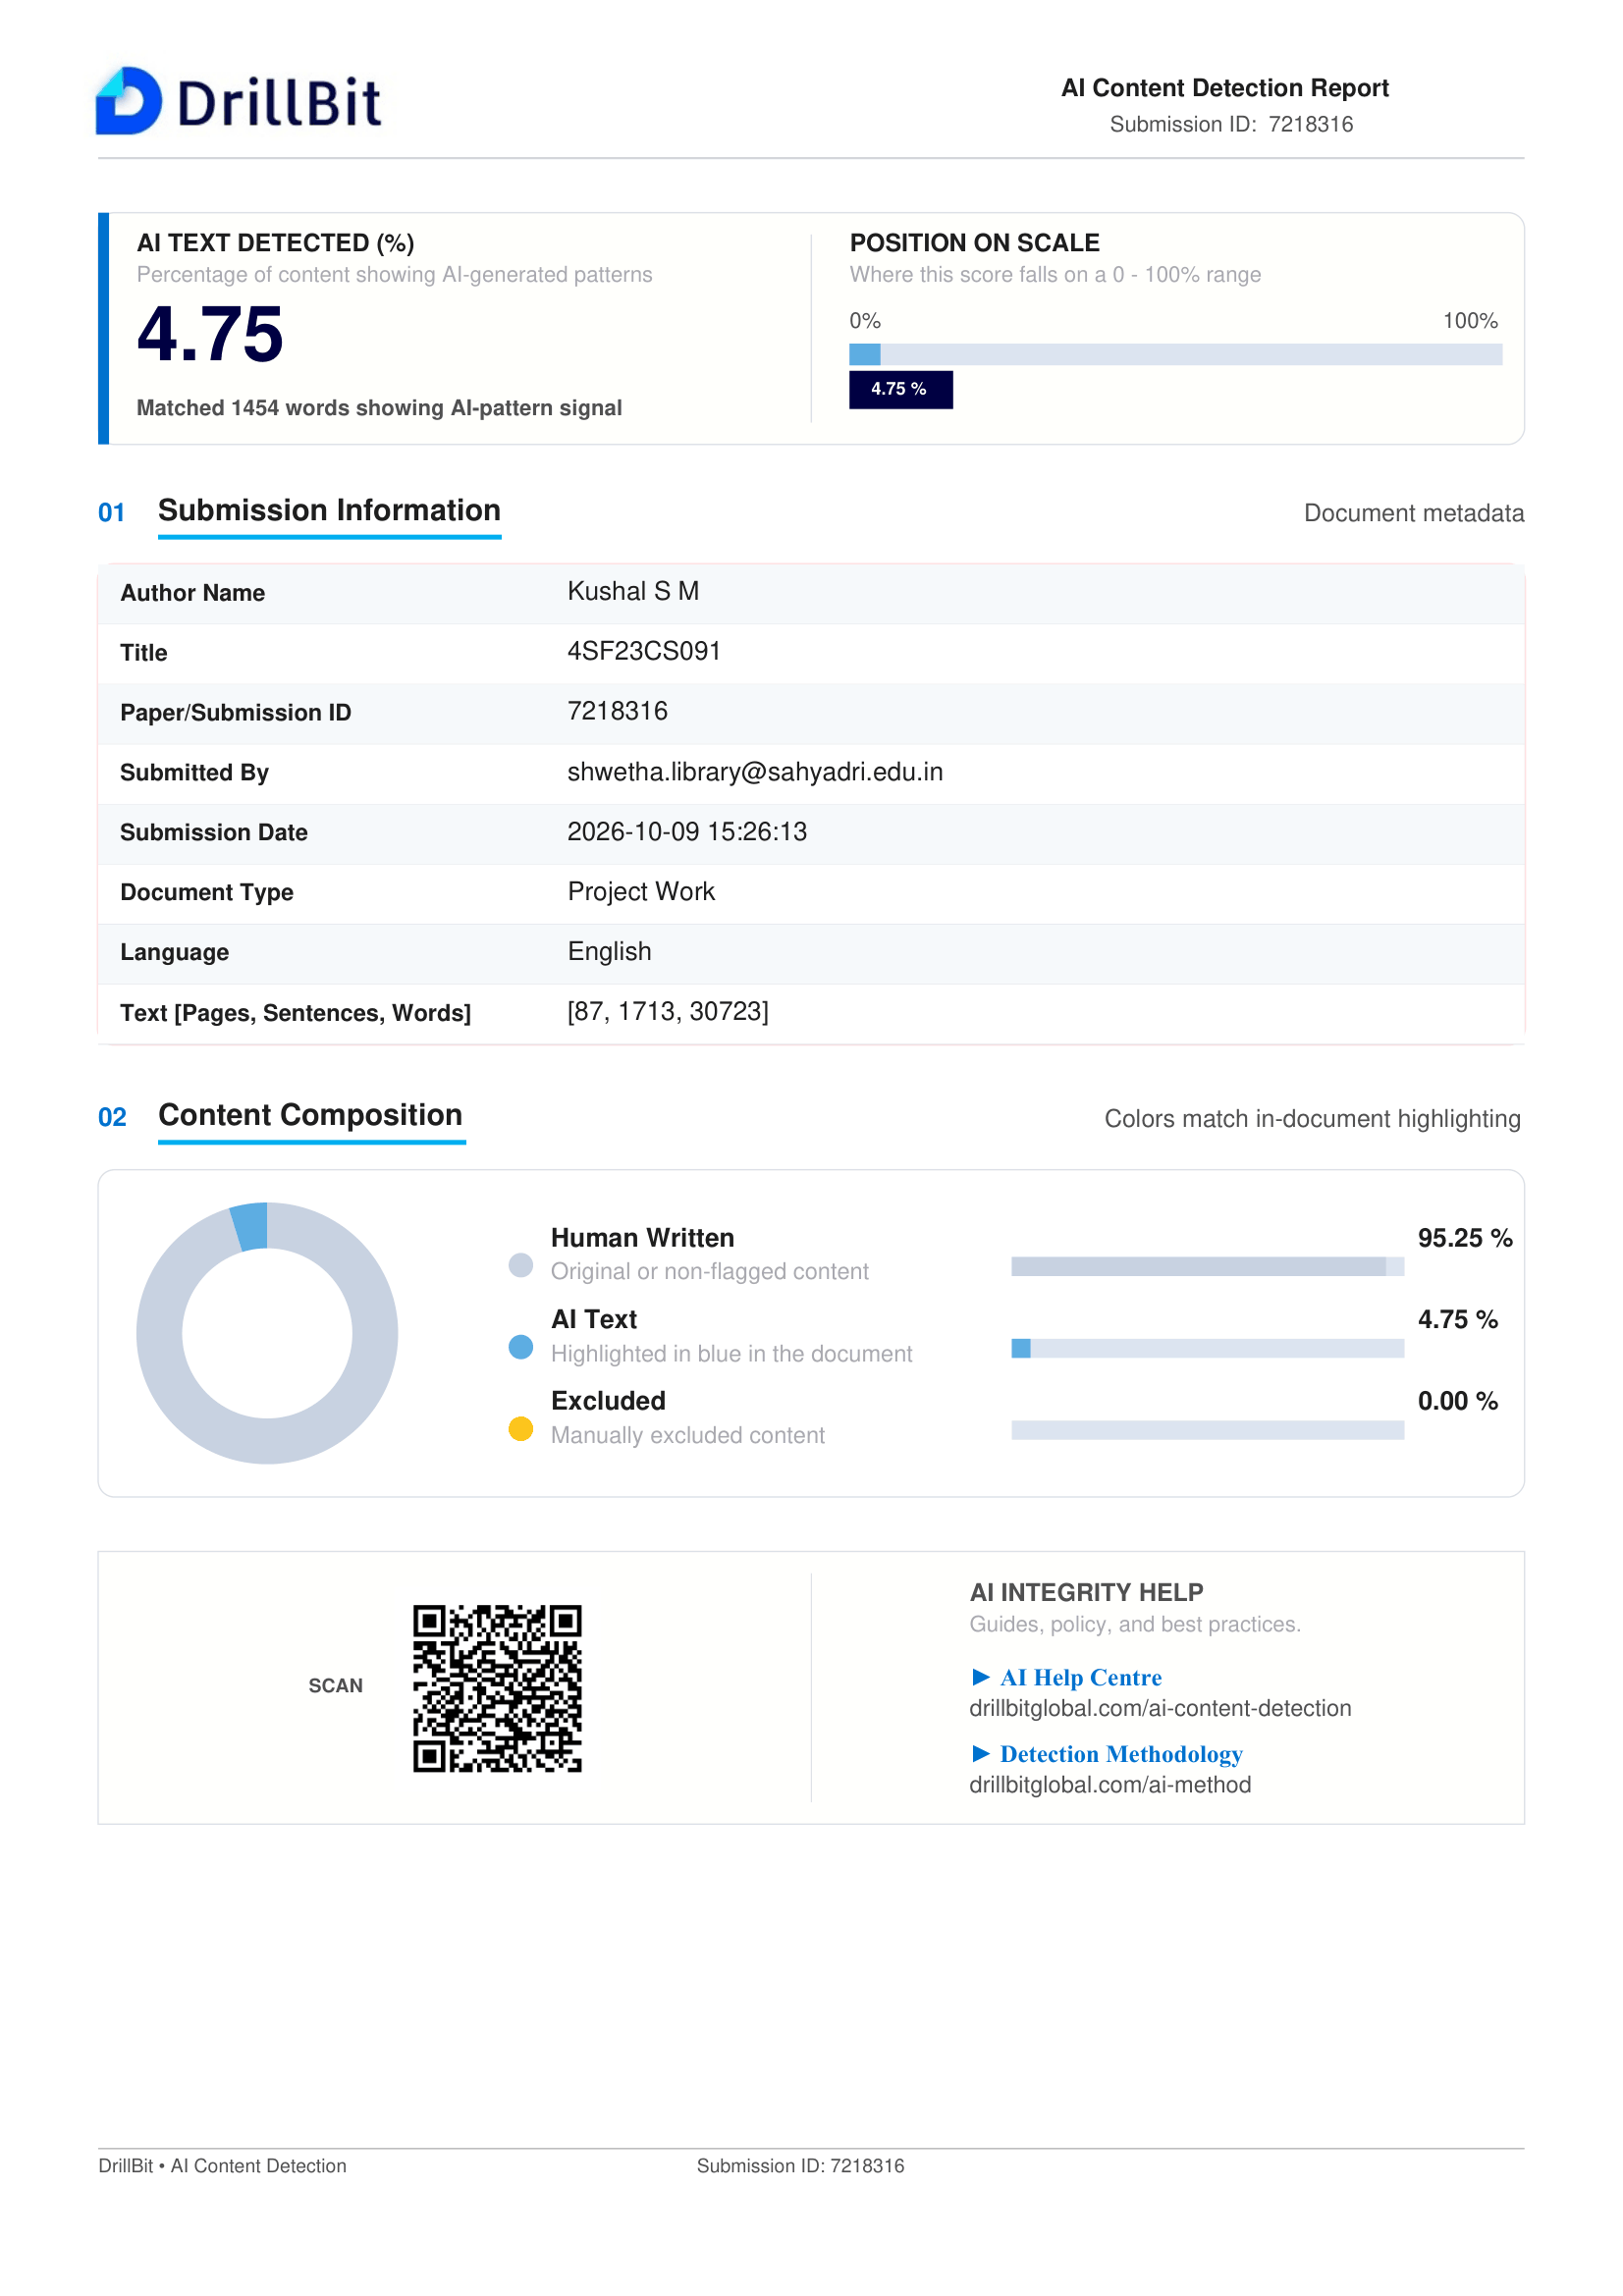
\includegraphics[width=0.94\textwidth,height=0.84\textheight,keepaspectratio]{AI_report}}
\end{center}

% ===========================================================================
\clearpage
\chapter[Paper Publication Details]{Paper Publication Details}
\thispagestyle{plain}
\begin{center}
\fbox{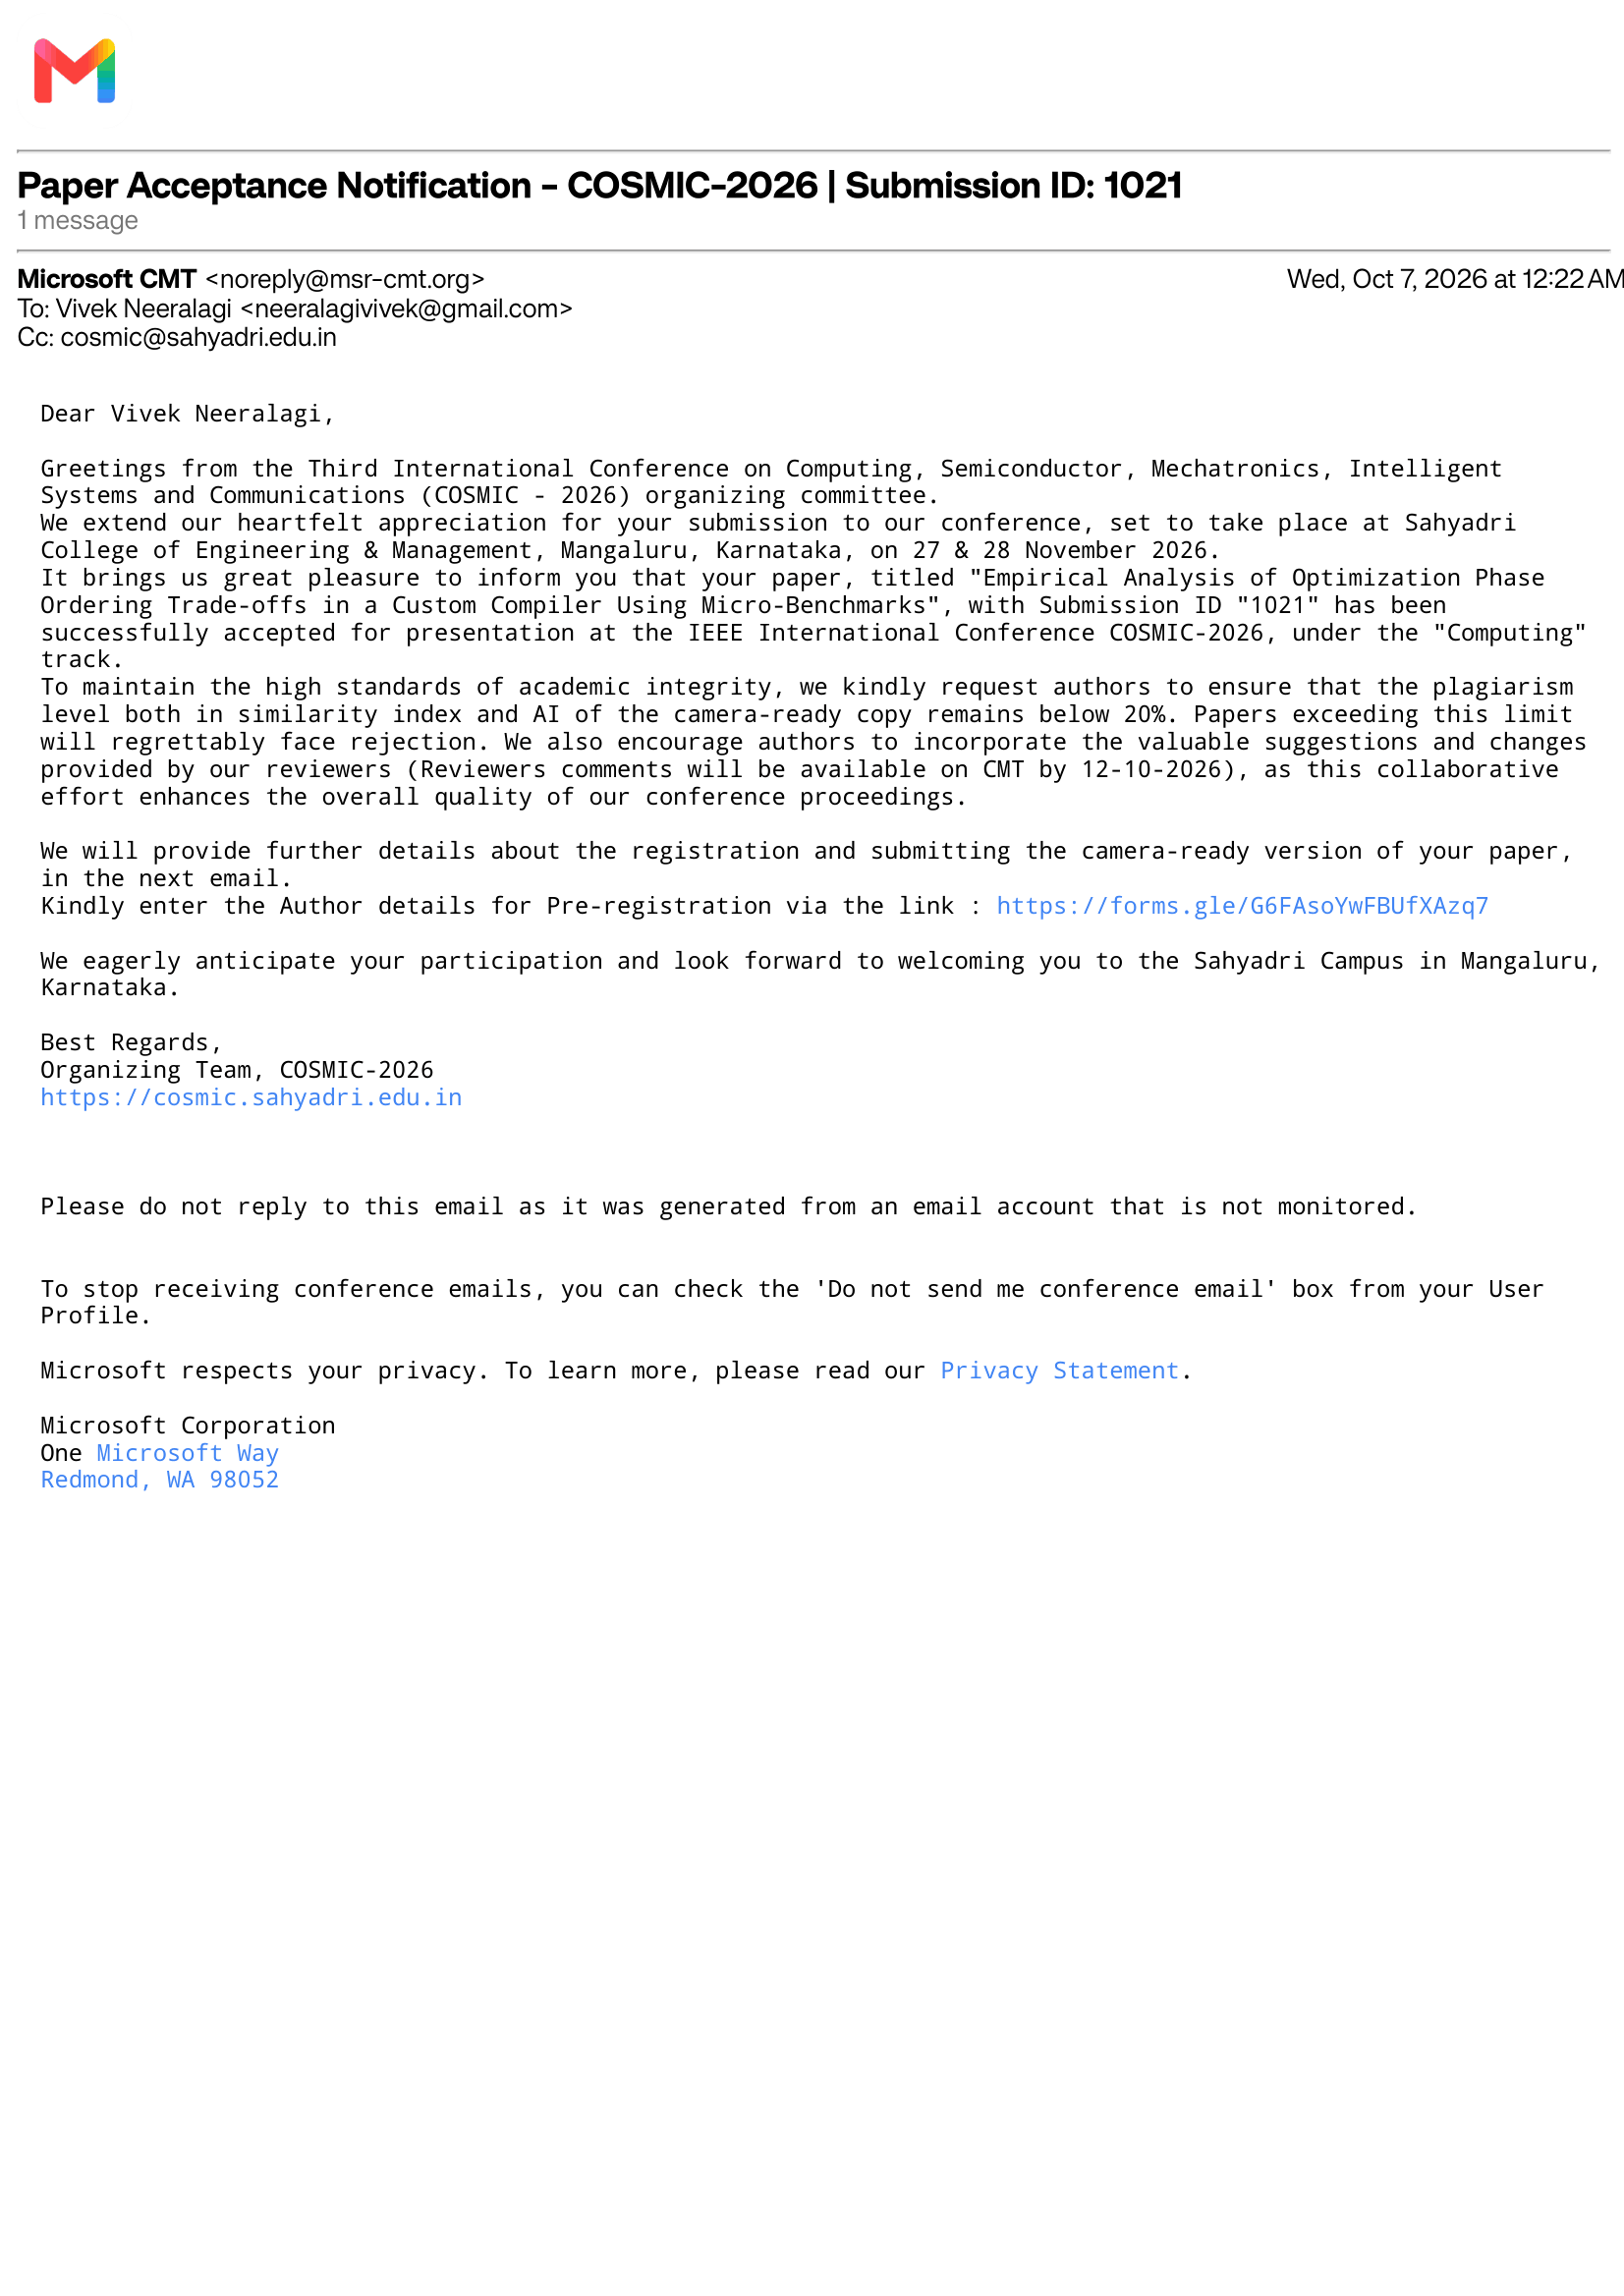
\includegraphics[width=\textwidth,height=0.78\textheight,keepaspectratio]{paper-acceptance}}
\end{center}

% ===========================================================================
\clearpage
\chapter[Paper Copy]{Paper Copy}
\thispagestyle{plain}
\begin{center}
\fbox{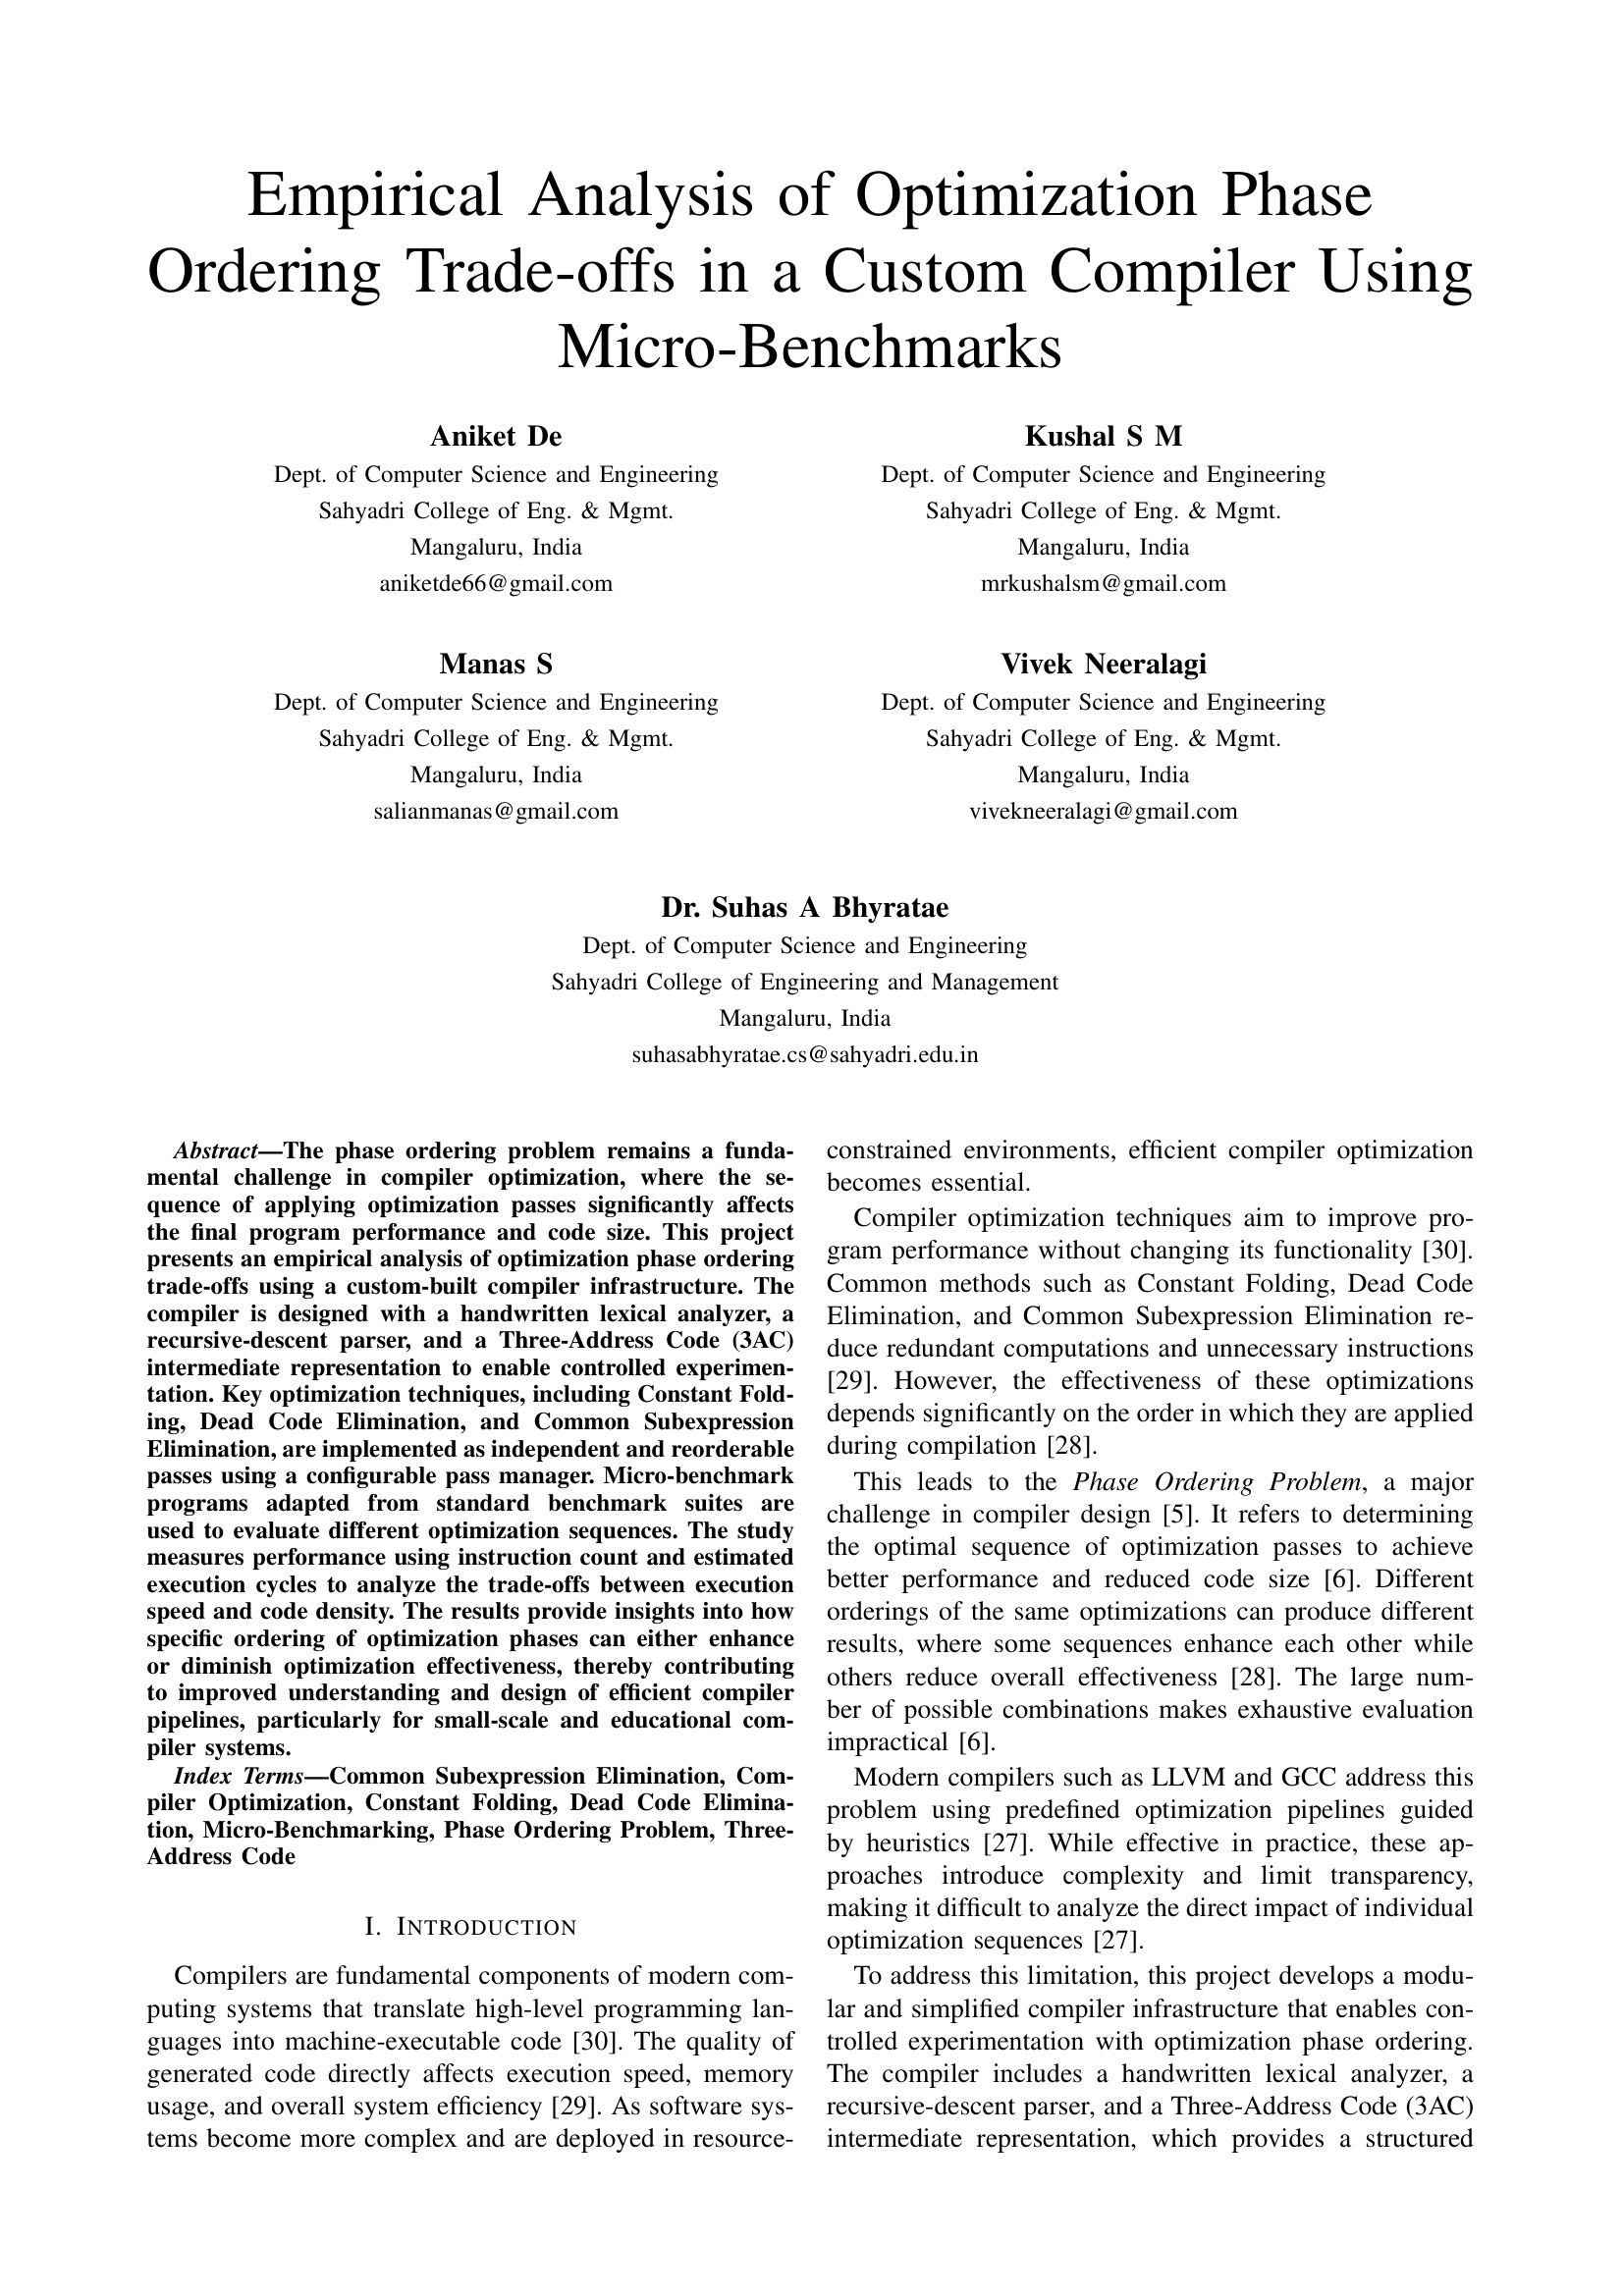
\includegraphics[width=0.94\textwidth,height=0.77\textheight,keepaspectratio]{paper-1}}
\end{center}

% ===========================================================================
\clearpage
\chapter[Code Snippets of Major Modules]{Code Snippets of Major Modules}
\thispagestyle{plain}

The excerpts below are taken verbatim from the project repository and show the core of each major module. Docstrings and explanatory comments present in the source have been shortened where marked with an ellipsis; no code has been changed.

\snippet{Pass manager: applying an ordering and enumerating all orderings}{compiler/optimizations/pass\_manager.py}{class \code{PassManager}}
\begin{lstlisting}[style=snippet]
    def run(self, instructions: list[IRInstruction]) -> list[IRInstruction]:
        """Apply the pass sequence to the IR and return the optimized result."""
        result = list(instructions)  # don't mutate original
        for name in self.pass_names:
            pass_fn = PASS_REGISTRY[name]
            result = pass_fn(result)
        return result

    @staticmethod
    def all_full_orderings(pass_names: list[str] | None = None) -> list[list[str]]:
        """Generate only the full-length permutations (all passes used)."""
        if pass_names is None:
            pass_names = list(PASS_REGISTRY.keys())

        orderings: list[list[str]] = [[]]  # baseline
        for perm in permutations(pass_names):
            orderings.append(list(perm))
        return orderings
\end{lstlisting}

\snippet{Constant folding: folding and propagating through one instruction}{compiler/optimizations/constant\_folding.py}{function \code{\_fold\_instruction}}
\begin{lstlisting}[style=snippet]
def _fold_instruction(inst: IRInstruction, const_map: dict[str, str]) -> IRInstruction:
    """Try to fold a single instruction using known constants."""
    opcode = inst.opcode

    # --- Binary operations ---
    if opcode in _BINARY_OPCODES:
        s1 = _resolve(inst.src1, const_map)
        s2 = _resolve(inst.src2, const_map)

        if s1 is not None and s2 is not None and is_constant(s1) and is_constant(s2):
            fn = _EVAL_OPS[opcode]
            val = fn(const_value(s1), const_value(s2))
            return IRInstruction(IROpcode.LOAD_CONST, inst.dest, str(int(val)))

        # Even if we can't fully fold, propagate constants into operands
        new_src1 = s1 if s1 != inst.src1 else inst.src1
        new_src2 = s2 if s2 != inst.src2 else inst.src2
        if new_src1 != inst.src1 or new_src2 != inst.src2:
            return IRInstruction(opcode, inst.dest, new_src1, new_src2)
        return inst
    # ... unary operations, COPY, array and global stores, and
    #     conditional jumps on constants are handled the same way
\end{lstlisting}

\snippet{Dead code elimination: fixed-point removal of unread definitions}{compiler/optimizations/dead\_code\_elimination.py}{functions \code{\_remove\_dead\_assignments} and \code{\_is\_dead}}
\begin{lstlisting}[style=snippet]
def _remove_dead_assignments(instructions: list[IRInstruction]) -> list[IRInstruction]:
    """Iteratively remove assignments to variables that are never read."""
    changed = True
    working = list(instructions)

    while changed:
        changed = False

        # Collect all used variables
        used: set[str] = set()
        for inst in working:
            used |= inst.used_vars()

        new_working: list[IRInstruction] = []
        for inst in working:
            if _is_dead(inst, used):
                changed = True
            else:
                new_working.append(inst)

        working = new_working

    return working


def _is_dead(inst: IRInstruction, used: set[str]) -> bool:
    """Determine if an instruction is dead (defines an unused variable
    and has no side effects)."""
    # Never remove these - they have side effects or structural meaning.
    if inst.opcode in (
        IROpcode.PRINT, IROpcode.RETURN, IROpcode.PARAM,
        IROpcode.JUMP, IROpcode.JUMP_IF_TRUE, IROpcode.JUMP_IF_FALSE,
        IROpcode.LABEL, IROpcode.FUNC_BEGIN, IROpcode.FUNC_END,
        IROpcode.CALL,  # calls may have side effects
        IROpcode.ARR_DECL, IROpcode.ARR_STORE,
        IROpcode.GLOBAL_DECL, IROpcode.GLOBAL_STORE,
        IROpcode.NOP,
    ):
        return False

    defined = inst.defined_var()
    if defined is None:
        return False

    # A temp or variable that nobody reads is dead
    return defined not in used
\end{lstlisting}

\snippet{Common subexpression elimination: the available-expression table}{compiler/optimizations/common\_subexpression\_elimination.py}{main loop of the pass function}
\begin{lstlisting}[style=snippet]
    for inst in instructions:
        # Control flow boundaries: conservatively clear available expressions
        if inst.opcode in (
            IROpcode.LABEL, IROpcode.JUMP, IROpcode.JUMP_IF_TRUE,
            IROpcode.JUMP_IF_FALSE, IROpcode.CALL,
            IROpcode.FUNC_BEGIN, IROpcode.FUNC_END,
        ):
            available_exprs.clear()
            var_to_expr_keys.clear()
            result_var_to_expr_keys.clear()
            result.append(inst)
            continue

        if inst.opcode in _CSE_OPCODES and inst.dest:
            # Redefining dest invalidates expressions that depended on it,
            # and expressions previously associated with dest as a result.
            _invalidate_var(inst.dest, available_exprs,
                            var_to_expr_keys, result_var_to_expr_keys)

            expr_key = (inst.opcode, inst.src1, inst.src2)

            if expr_key in available_exprs:
                # Reuse the previously computed value
                prev_var = available_exprs[expr_key]
                result.append(IRInstruction(IROpcode.COPY, inst.dest, prev_var))
            else:
                result.append(inst)

            # Record where this expression is currently available.
            _set_available_expr(expr_key, inst.dest,
                                available_exprs, result_var_to_expr_keys)

            # Track operand -> expression key mapping for invalidation
            for operand in (inst.src1, inst.src2):
                if operand and not is_constant(operand):
                    var_to_expr_keys.setdefault(operand, set()).add(expr_key)
            continue

        # For other instructions, check if they redefine a variable
        defined = inst.defined_var()
        if defined:
            _invalidate_var(defined, available_exprs,
                            var_to_expr_keys, result_var_to_expr_keys)

        result.append(inst)

    return result
\end{lstlisting}

\snippet{Copy propagation: recording copies and substituting operands}{compiler/optimizations/copy\_propagation.py}{main loop of the pass function}
\begin{lstlisting}[style=snippet]
    for inst in instructions:
        # Control-flow boundaries: conservatively clear
        if inst.opcode in (
            IROpcode.LABEL, IROpcode.JUMP, IROpcode.JUMP_IF_TRUE,
            IROpcode.JUMP_IF_FALSE, IROpcode.CALL,
            IROpcode.FUNC_BEGIN, IROpcode.FUNC_END,
        ):
            copy_map.clear()
            result.append(inst)
            continue

        # Record COPY instructions: dest = src
        if inst.opcode == IROpcode.COPY and inst.dest and inst.src1:
            resolved_src = _resolve(inst.src1, copy_map)   # follow the copy chain
            _invalidate(inst.dest, copy_map)                # dest gets a new value
            copy_map[inst.dest] = resolved_src
            result.append(IRInstruction(IROpcode.COPY, inst.dest, resolved_src))
            continue

        # For LOAD_CONST, the dest gets a new value - record it as a
        # constant "copy" so downstream uses can be substituted
        if inst.opcode == IROpcode.LOAD_CONST and inst.dest and inst.src1:
            _invalidate(inst.dest, copy_map)
            copy_map[inst.dest] = inst.src1
            result.append(inst)
            continue

        # Substitute operands in all other instructions
        new_inst = _substitute(inst, copy_map)

        # If this instruction defines a variable, invalidate its copy entry
        defined = new_inst.defined_var()
        if defined:
            _invalidate(defined, copy_map)

        result.append(new_inst)

    return result
\end{lstlisting}

\snippet{Metric collector: the cost model and the two static metrics}{compiler/benchmarks/metric\_collector.py}{cost table and the two static metric functions}
\begin{lstlisting}[style=snippet]
INSTRUCTION_COST: dict[IROpcode, float] = {
    # Arithmetic - single-cycle ALU
    IROpcode.ADD:        1.0,
    IROpcode.SUB:        1.0,
    IROpcode.MUL:        3.0,    # multiply is typically 3 cycles
    IROpcode.DIV:        12.0,   # division is expensive
    IROpcode.MOD:        12.0,
    # ... comparisons, logical operations, COPY and LOAD_CONST: 1.0
    # Control flow
    IROpcode.JUMP:           2.0,   # branch penalty
    IROpcode.JUMP_IF_TRUE:   2.0,
    IROpcode.JUMP_IF_FALSE:  2.0,
    IROpcode.LABEL:          0.0,   # not a real instruction
    # Function operations
    IROpcode.PARAM:      1.0,
    IROpcode.CALL:       5.0,   # call overhead
    IROpcode.RETURN:     3.0,   # return overhead
    # I/O
    IROpcode.PRINT:      10.0,  # I/O is slow
    # Arrays and globals - memory access, costed like LDR/STR
    IROpcode.ARR_LOAD:   2.0,
    IROpcode.ARR_STORE:  2.0,
    IROpcode.GLOBAL_LOAD:  2.0,
    IROpcode.GLOBAL_STORE: 2.0,
    # ... declarations, function markers and NOP: 0.0
}


def count_code_size(instructions: list[IRInstruction]) -> int:
    """Count meaningful instructions (exclude labels, NOPs, structural markers)."""
    skip = {IROpcode.LABEL, IROpcode.NOP, IROpcode.FUNC_BEGIN, IROpcode.FUNC_END,
            IROpcode.FUNC_PARAM, IROpcode.GLOBAL_DECL}
    return sum(1 for inst in instructions if inst.opcode not in skip)


def estimate_cycles(instructions: list[IRInstruction]) -> float:
    """Estimate total execution cost using the weighted cost model."""
    return sum(INSTRUCTION_COST.get(inst.opcode, 1.0) for inst in instructions)
\end{lstlisting}

\snippet{IR interpreter: arithmetic dispatch table and control-flow execution}{compiler/interpreter.py}{dispatch table and the body of \code{\_execute\_function}}
\begin{lstlisting}[style=snippet]
# Binary operation dispatch table
_BINARY_OPS: dict[IROpcode, object] = {
    IROpcode.ADD: lambda a, b: a + b,
    IROpcode.SUB: lambda a, b: a - b,
    IROpcode.MUL: lambda a, b: a * b,
    IROpcode.DIV: lambda a, b: a // b if b != 0 else 0,
    IROpcode.MOD: lambda a, b: a % b if b != 0 else 0,
    IROpcode.EQ:  lambda a, b: int(a == b),
    IROpcode.NEQ: lambda a, b: int(a != b),
    IROpcode.LT:  lambda a, b: int(a < b),
    IROpcode.GT:  lambda a, b: int(a > b),
    IROpcode.LTE: lambda a, b: int(a <= b),
    IROpcode.GTE: lambda a, b: int(a >= b),
    IROpcode.AND: lambda a, b: int(bool(a) and bool(b)),
    IROpcode.OR:  lambda a, b: int(bool(a) or bool(b)),
}

# ... inside _execute_function, one branch per opcode:
            if inst.opcode == IROpcode.JUMP:
                pc = self._label_index[inst.dest]
                continue

            if inst.opcode == IROpcode.JUMP_IF_FALSE:
                if not self._get_value(inst.src1):
                    pc = self._label_index[inst.dest]
                else:
                    pc += 1
                continue

            if inst.opcode == IROpcode.PARAM:
                # Collect params for upcoming CALL
                if not hasattr(self, '_pending_params'):
                    self._pending_params: list[int] = []
                self._pending_params.append(self._get_value(inst.src1))
                pc += 1
                continue

            if inst.opcode == IROpcode.CALL:
                params = getattr(self, '_pending_params', [])
                self._pending_params = []
                ret = self._execute_function(inst.src1, params)
                self._vars[inst.dest] = ret
                pc += 1
                continue

            if inst.opcode == IROpcode.RETURN:
                if inst.src1:
                    return_value = self._get_value(inst.src1)
                break

            if inst.opcode == IROpcode.PRINT:
                val = self._get_value(inst.src1)
                self._output.append(val)
                pc += 1
                continue
\end{lstlisting}

\snippet{RISC-V RV32IM back end: guarded division and array access lowering}{compiler/codegen\_riscv.py}{method \code{\_gen\_instruction}}
\begin{lstlisting}[style=snippet]
        if op in (IROpcode.DIV, IROpcode.MOD):
            mnemonic = "div" if op == IROpcode.DIV else "rem"
            zero_l = self._label("divz")
            done_l = self._label("divdone")
            self._load("t0", inst.src1)
            self._load("t1", inst.src2)
            self._emit(f"    beqz t1, {zero_l}")
            self._emit(f"    {mnemonic} t2, t0, t1")
            self._emit(f"    j {done_l}")
            self._emit(f"{zero_l}:")
            self._emit("    li t2, 0               # x/0 == 0 by language rule")
            self._emit(f"{done_l}:")
            self._store("t2", inst.dest)
            return
        if op == IROpcode.ARR_LOAD:
            self._load("t0", inst.src2)          # index
            self._emit("    slli t0, t0, 2")
            self._array_base("t1", inst.src1)
            self._emit("    add t1, t1, t0")
            self._emit("    lw t2, 0(t1)")
            self._store("t2", inst.dest)
            return
        if op == IROpcode.ARR_STORE:
            self._load("t0", inst.src1)          # index
            self._emit("    slli t0, t0, 2")
            self._array_base("t1", inst.dest)
            self._emit("    add t1, t1, t0")
            self._load("t2", inst.src2)          # value
            self._emit("    sw t2, 0(t1)")
            return
\end{lstlisting}
